\documentclass{article}

\usepackage{graphicx}
\usepackage{tikz}
\usepackage{tikzsymbols}
\usetikzlibrary{calc,patterns,shapes.geometric}
\pagestyle{empty}
\usepackage[margin=0pt]{geometry}
\geometry{papersize={14in,12in}}

\def\centerarc[#1](#2)(#3:#4:#5){\draw[#1] ($(#2)+({#5*cos(#3)},{#5*sin(#3)})$) arc (#3:#4:#5);}

\begin{document}
	\begin{figure}
		\centering
		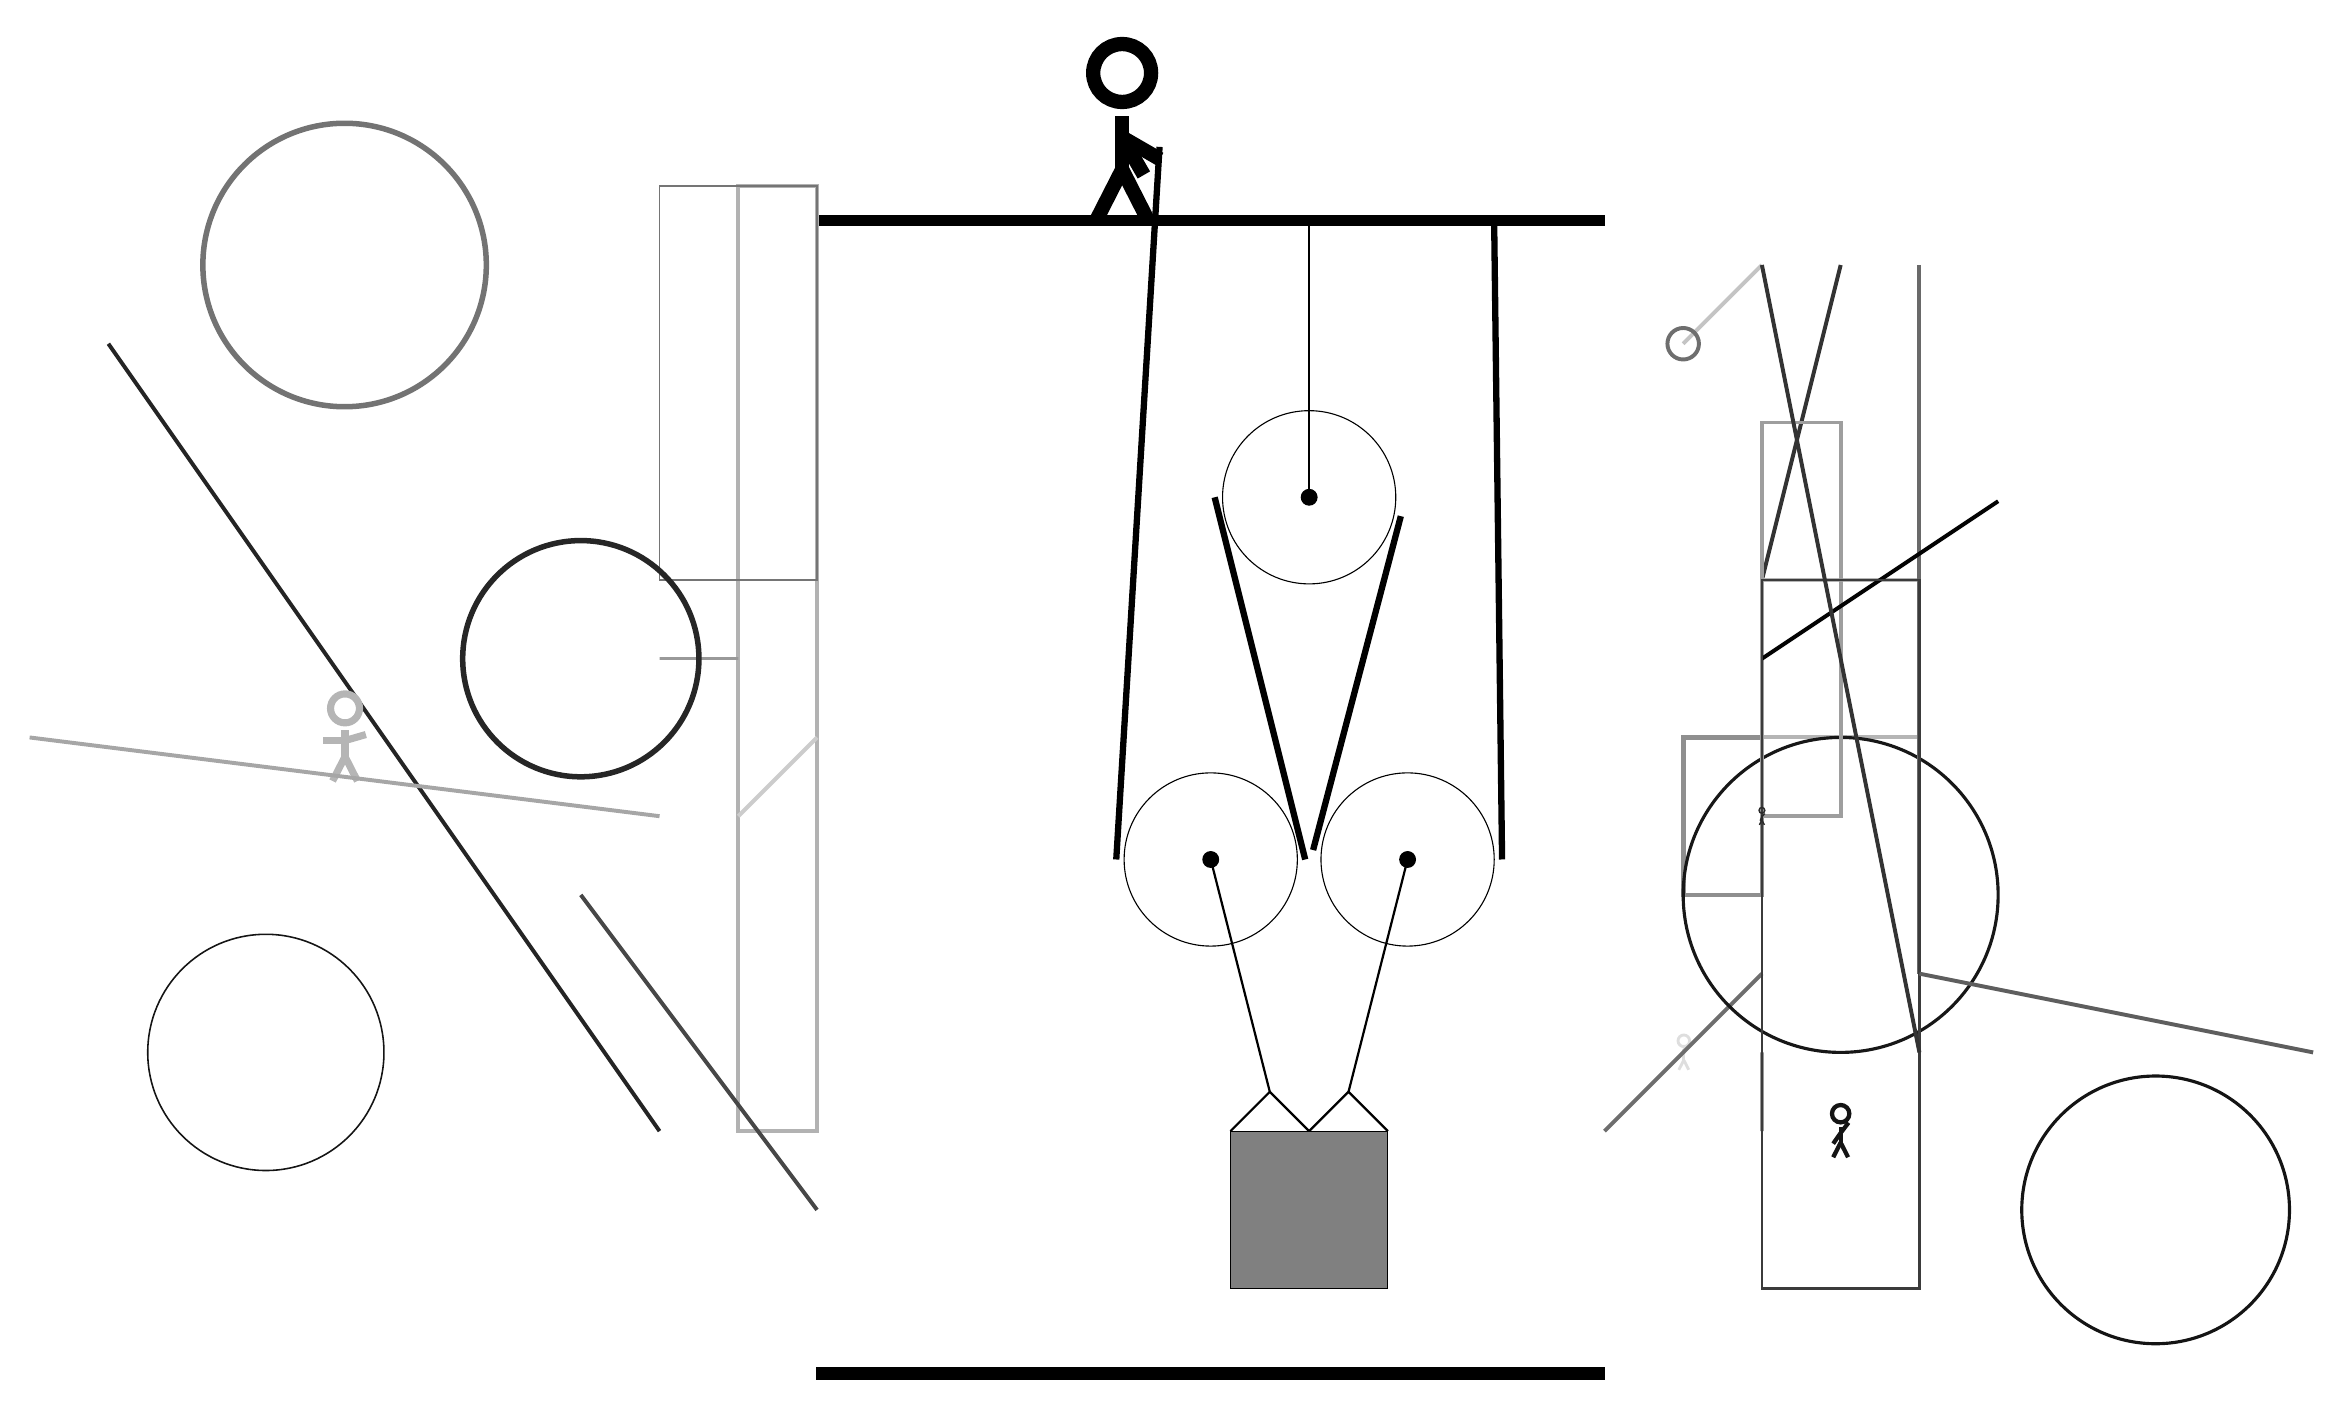
\begin{tikzpicture}
			%%%%% START %%%%%
			
			\draw[fill=black] (-4, 11.5) rectangle (6, 11.625);
			
			\draw (1, 3.45) circle (1.1);
			\draw[fill=black] (1, 3.45) circle (0.1);
			
			\draw (2.25, 8.05) circle (1.1);
			\draw[fill=black] (2.25, 8.05) circle (0.1);
			\draw[thick] (2.25, 8.05) -- (2.25, 11.5);
			
			\draw (3.5, 3.45) circle (1.1);
			\draw[fill=black] (3.5, 3.45) circle (0.1);
			
			\draw[line width=0.5mm, color=black!80](8, 7) -- (9, 11);
			
			\draw[line width=0.5mm, color=black!30] (-4, 0) rectangle (-5, 12);
			\node[line width=0.7mm, color=black!13] at (7, 1) {\Strichmaxerl[2][36][83]};
			\draw[line width=0.5mm, color=black!20](-5, 4) -- (-4, 5);
			\draw[line width=0.6mm, color=black!35] (8, 9) rectangle (8, 3);
			\draw[line width=0.6mm, color=black!44] (8, 3) rectangle (7, 5);
			\draw [line width=0.4mm, color=black!92](13, -1) circle (1.7);
			\draw[line width=0.4mm, color=black!40] (-5, 6) rectangle (-6, 6);
			\draw [line width=0.2mm, color=black!92](-11, 1) circle (1.5);
			\draw[line width=0.5mm, color=black!23](7, 10) -- (8, 11);
			
			\draw [line width=0.5mm, color=black!57](7, 10) circle (0.2);
			
			\draw[line width=0.5mm, color=black!86](-6, 0) -- (-13, 10);
			\draw[line width=0.5mm, color=black!57](8, 2) -- (6, 0);
			
			\draw[line width=0.5mm, color=black!29] (8, 7) rectangle (10, 5);
			\node[line width=0.4mm, color=black!29] at (-10, 5) {\Strichmaxerl[5][0][16]};
			\draw [line width=0.7mm, color=black!55](-10, 11) circle (1.8);
			\draw[line width=0.5mm, color=black!72](-7, 3) -- (-4, -1);
			\node[line width=0.6mm, color=black!92] at (9, 0) {\Strichmaxerl[3][55][53]};
			\draw [line width=0.4mm, color=black!91](9, 3) circle (2.0);
			\draw[line width=0.5mm, color=black!59](10, 11) -- (10, 2);
			\draw[line width=0.5mm, color=black!35](-6, 4) -- (-14, 5);
			
			\draw[line width=0.6mm, color=black!40] (8, 0) rectangle (8, 1);
			\draw[line width=0.5mm, color=black!38] (8, 9) rectangle (9, 4);
			\draw[line width=0.2mm, color=black!54] (-6, 12) rectangle (-4, 7);
			\draw[line width=0.5mm, color=black!99](8, 6) -- (11, 8);
			\draw[line width=0.3mm, color=black!77] (8, 7) rectangle (10, -2);
			
			\draw[line width=0.5mm, color=black!63](10, 2) -- (15, 1);
			\draw[line width=0.5mm, color=black!80](8, 11) -- (10, 1);
			\node[line width=0.5mm, color=black!84] at (8, 4) {\Strichmaxerl[1][66][49]};
			\draw [line width=0.7mm, color=black!85](-7, 6) circle (1.5);
			
			\draw[thick] (3.5, 3.45) -- (2.75, 0.5);
			\draw[thick] (1, 3.45) -- (1.75, 0.5);
			\draw[thick]  (1.25, 0) -- (1.75, 0.5) -- (2.25, 0);
			\draw[thick]  (2.25, 0) -- (2.75, 0.5) -- (3.25, 0);
			\draw[fill=black!50] (1.25, 0) rectangle (3.25, -2);
			
			\draw[line width=0.8mm] (0.35, 12.5) --  (-0.2, 3.45);
			\centerarc[line width=0.8mm](1, 3.45)(180:360:1.2000000000000002);
			\draw[line width=0.8mm] (2.2, 3.45) -- (1.05, 8.05);
			\centerarc[line width=0.8mm](2.25, 8.05)(-20:180:1.2000000000000002);
			\draw[line width=0.8mm](3.414, 7.81) -- (2.3, 3.57);
			\centerarc[line width=0.8mm](3.5, 3.45)(160:360:1.2000000000000002);
			\draw[line width=0.8mm](4.7, 3.45) -- (4.6, 11.5);
			
			\node at (-0.07, 12.7) {\Strichmaxerl[10][120][-30]};
			
			\draw[fill=black] (-4, -3) rectangle (6, -3.15);
			
			%%%%% END %%%%%
		\end{tikzpicture}
	\end{figure}	
\end{document}